\section{Hardness Results}

We consider several variants of the Boolean matrix factorization problem:
 given a symmetric square matrix $B \in \Z^{n \times n}$, find $A \in \{0,1\}^{n \times m}$ such that $B=AA^T$ or similar conditions.
We here use Feldmann et al.'s notation \cite{feldmann_fixed-parameter_2020}.
%
We allow matrices to have wildcard entries in the diagonal that will be denoted by $\star$.
We define $\Z^\star := \Z_{\geq 0} \cup \{\star\}$.
For $x, y \in \Z$, we write $x \stackrel{\star}{=} y$ if and only if either $x=y$, or at least one of $x$ and $y$ is $\star$.
For two matrices $X$ and $Y$ in $(\Z^\star)^{m\times n}$, we write $X \stackrel{\star}{=} Y$
 if and only if $X_{i,j} \stackrel{\star}{=} Y_{i,j}$ for all $i$, $j$.
Further, $\|\cdot\|_0$ denotes the number of nonzero entries.
%
\Cref{tab:hardness} summarizes known and newly established hardness results.

\begin{table*}[ht]
  \centering
  \small

  \begin{tabular}{|c|c|p{0.18\textwidth}|p{0.18\textwidth}|p{0.3\textwidth}|p{0.18\textwidth}|}
    \hline
    \#
    &Given
    &\multicolumn{1}{c|}{Given $B$} 
    &\multicolumn{1}{c|}{Find $A$} 
    &\multicolumn{1}{c|}{Problem / Interpretation}
    &\multicolumn{1}{c|}{Hardness}
    \\
    \hline
    (1) & $m \in \N$ & $B \in \{0,1,\star \}^{n \times n}$,\newline $b_{i,i}=\star\quad\forall i$
     & $A \in \{0,1\}^{n \times m}$,\newline $B\stackrel{\star}{=}AA^T$
     & Edge Clique Partition of a graph with $n$ vertices; decompose all edges into a set of $m$ cliques (if such one exists).
     & NP-hard \cite{shaohan1988complexity}\\
    \hline
    (2) & $m \in \N$ & $B \in (\Z^\star)^{n \times n}$,\newline $b_{i,i}=\star \quad\forall i$
     & $A \in \{0,1\}^{n \times m}$,\newline $B\stackrel{\star}{=}AA^T$
     & Weighted Edge Clique Partition of a graph with $n$ vertices
     (equivalently, Edge Clique Partition on a multigraph without loops);
     decompose all weighted edges into a multiset of $m$ cliques.
     & NP-hard \cite{feldmann_fixed-parameter_2020,cooley_parameterized_2021}\\
    \hline
    (3) & $m \in \N$ & $B \in \Z^{n \times n}$
    & $A \in \{0,1\}^{n \times m}$,\newline $B=AA^T$
    & (a) Weighted Clique Decomposition of a hypergraph with $n$ vertices and $m$ hyperedges.
    (b) Recovering a hypergraph with $m$ vertices and $n$ hyperedges from the given weighted line graph.
    & \textcolor{blue}{NP-hard}\\
    \hline
    (4) & --- & $B \in (\Z^\star)^{n \times n}$,\newline $b_{i,i}=\star \quad\forall i$
    & $A \in \{0,1\}^{n \times m}$,\newline $B\stackrel{\star}{=}AA^T$
    & (a) Weighted Clique Decomposition of a hypergraph with $n$ vertices 
    and \textit{any number of} hyperedges, \textbf{ignoring the diagonal entries in $B$ (vertex weights)}.
    (b) Recovering a hypergraph with \textit{any number of} vertices and 
    $n$ hyperedges from the given weighted line graph, ignoring the diagonal entries in $B$.
    & \textcolor{blue}{P}\\
    \hline
    (5) & --- & $B \in \Z^{n \times n}$
    & $A \in \{0,1\}^{n \times m}$,\newline $B=AA^T$
    & (a) Weighted Clique Decomposition of a hypergraph with $n$ vertices and \textit{any number of} hyperedges.
    (b) Recovering a hypergraph with \textit{any number of} vertices and $n$ hyperedges from the given weighted line graph.
    & Open? Literature survey needed.\\
    \hline
    (6) & $k \in \N$ & $B \in \Z^{n \times n}$
    & $A \in \{0,1\}^{n \times m}$,\newline 
    $\|A_{i,*}\|_0=k\quad\forall i$,\newline
    $B=AA^T$
    & (a) Weighted Clique Decomposition of a $k$-\textbf{regular} hypergraph with $n$ vertices.
    (b) Recovering a $k$-\textbf{uniform} hypergraph with $n$ hyperedges from the given weighted line graph.
    & P when $k=2$ \cite{roussopoulos_max_1973,lehot_optimal_1974,syslo_labeling_1982,degiorgi_dynamic_1995,liu_iligra_2015};\newline
    NP-hard when $k \geq 3$ \cite{poljak_complexity_1981,chen_symmetric_2022}\\
    \hline
    (7) & $k \in \N$ & $B \in \Z^{n \times n}$
    & $A \in \{0,1\}^{n \times m}$,\newline 
    $\|A_{*,j}\|_0=k\quad \forall j$,\newline
    $B=AA^T$
    & (a) Weighted Clique Decomposition of a $k$-\textbf{uniform} hypergraph with $n$ vertices.
    (b) Recovering a $k$-\textbf{regular} hypergraph with $n$ hyperedges from the given weighted line graph.
    & Open? Literature survey needed.\\
    \hline
  \end{tabular}

  \caption{%
  Known and established hardness results (new results in blue).
  }
  \label{tab:hardness}
\end{table*}


\begin{thm}\label{thm:hardness-bounded}
  Problem (3) in \Cref{tab:hardness} is NP-hard.
\end{thm}

\begin{proof}[Proof Sketch of Theorem~\ref{thm:hardness-bounded}]
  We use the same construction as given by \cite{cooley_parameterized_2021,shaohan1988complexity}.
  We will show that Problem (3) in \Cref{tab:hardness} is NP-hard by a reduction from 
  \textsc{Exact Cover by 3-Sets (X3C)}.
  In this problem, we are given a universe $U$ of $3q$ elements and a collection
  $\mathcal{S}=\{S_1,S_2,\ldots,S_\ell\}$ of $\ell$ 3-ary subsets of $U$.
  The decision problem asks whether there exist $q$ sets in $\mathcal{S}$ that cover the entire $U$.
  % Without loss of generality, we assume $U=\{1,2,\ldots,3q\}$ and $S_i = \{x_i, y_i, z_i\}$ for each $i$.

  Given an instance of X3C, we construct an auxiliary graph $G$ as follows.
  %
  For each element $u\in U$, we introduce two vertices $u, u'$ and have an edge $uu'$ in $G$.
  We call these vertices and edges the \textit{element-vertices} and \textit{element-edges}, respectively.
  %
  For each set $S_i=\{u,v,w\}$ in $\mathcal{S}$, we will have three vertices $a_i, b_i, c_i$ that
  form a triangle. We call these vertices \textit{set-vertices}.
  Then, we connect this triangle to the element edges by adding the following 9 edges:
  $a_i u, a_i u', a_i v, b_i v, b_i v', b_i w, c_i w, c_i w', c_i u$.

  We now construct a matrix $B \in \Z^{n \times n}$, where each row/column corresponds to 
  a vertex in $G$. There are $n = 6q + 3\ell$ vertices.
  For every distinct $i, j$, let $b_{i,j} = 1$ if $G$ has an edge between $i$ and $j$;
  otherwise, $b_{i,j}=0$.
  Finally, for every element-vertex $u$, set $b_{u,u}=(\deg_G(u) + 1)/2$
  for $u'$, set $b_{u',u'}=\deg_G(u')-1$, and 
  for every set-vertex $u$, set $b_{u,u}=3$.
  %
  We set $m$, the number of cliques, to be $6\ell + q$.

  (X3C Yes-instance $\to$ Problem (3) Yes-instance)
  WLOG assume that $S_1,S_2,\ldots,S_q$ is a solution to X3C.
  %
  For each $1 \leq i \leq q$, take the 7 cliques
  $\{a_i, b_i, c_i\}, \{u, u', a_i\}, \{v, v', b_i\}, \{w, w', c_i\}, \{v, a_i\}, \{w, b_i\}, \{u, c_i\}$
  into the solution.
  %
  For each $q < i \leq \ell$, take the 6 cliques
  $\{v, a_i, b_i\}, \{w, b_i, c_i\}, \{u, c_i, a_i\}, \{u', a_i\}, \{v', b_i\}, \{w', c_i\}$
  into the solution.
  %
  This is a valid solution for Problem (3);
  there are $7q + 6(\ell - q) = 6\ell + q$ cliques.
  %
  Let $x=|\{S_i: q < i \leq \ell, u \in S_i \}|$.
  Element-vertex $u$ is included in $2 + x$ cliques,
  while $\deg_G(u)=3+2x$, satisfying $b_{u,u}=(\deg_G(u)+1)/2$.
  Element-vertex $u'$ is included in $1 + x$ cliques,
  while $\deg_G(u')=2+x$, satisfying $b_{u',u'}=\deg_G(u')-1$.
  %
  Each set-vertex $a_i$ ($b_i, c_i$) is included in exactly 3 cliques whether $i \leq q$ or not.
  Every edge in $G$ is covered by exactly one clique.

  (Problem (3) Yes-instance $\to$ X3C Yes-instance)
  For each $1 \leq i \leq \ell$, define\newline
  $E_i=\{a_ib_i, b_ic_i, c_ia_i, a_iu, a_iu, a_iv, b_iv, b_iv', b_iw, c_iw, c_iw', c_iu'\}$, the edges \textit{exclusive} to the set $S_i$.
  Let $\mathcal{C}$ be the set of cliques in the solution to Problem (3) when interpreted as cliques.
  Also, let $C_i=\{C \in \mathcal{C}: C \cap E_i \neq \emptyset\}$.
  Observe that if $C_i$ contains a clique including any element edge $uu'$, then $|C_i|\geq 7$,
  and $|C_i|\geq 6$, otherwise. It is easy to see $C_i \cap C_j=\emptyset$ for distinct $i,j$.
  %
  Since there are only $6\ell + q$ cliques, there are exactly $q$ sets that cover all element edges,
  which gives the required solution for X3C.
\end{proof}

\begin{thm}\label{thm:hardness-unbounded-ignore-diag}
  Problem (4) in \Cref{tab:hardness} can be solved in polynomial time in $n$.
\end{thm}

\begin{proof}[Proof Sketch of Theorem~\ref{thm:hardness-unbounded-ignore-diag}]
  Consider this problem as Weighted Clique Decomposition.
  %
  First, observe that adding a clique of size 1 does not change the feasibility
  because the diagonal entries in $B$ are ignored.
  If the instance is feasible, then there must exist a solution without a clique of size 1.
  %
  Therefore, it is enough to construct a set of cliques of size 2 in a greedy manner.
  %
  This construction will require $\sum_{1 \leq i < j \leq n}b_{i,j}$ cliques.
\end{proof}

\begin{thm}\label{thm:hardness-unbounded}
  Problem (5) in \Cref{tab:hardness} is NP-hard.
\end{thm}

\begin{proof}[Proof Sketch of Theorem~\ref{thm:hardness-unbounded}]
  We use the same construction as in the proof of Theorem~\ref{thm:hardness-bounded}.
  Given the construction of a $K_4$-free graph $G$, we claim that the number of cliques is
  determined by the diagonal entries of $B$.

  Let $y_i(u)$ be the number of cliques of size $i$ incident to vertex $u$.
  Because $G$ is $K_4$-free and all edges have unit weight, we have $b_{u,u} = y_1(u) + y_2(u) + y_3(u)$ and 
  $\deg_G(u) = y_2(u) + 2 y_3(u)$. Trivially, we get $\deg_G(u)-b_{u,u} \leq y_3(u) \leq \deg_G(u) /2$.

  For each element-vertex $u$, we have $b_{u,u}=(\deg_G(u)+1)/2$, so $y_3(u)=(\deg_G(u)-1)/2$,
  which then determines $y_1(u)=0$ and $y_2(u)=1$ (note that $\deg_G(u)$ is always odd).
  %
  For each element-vertex $u'$, we have $b_{u',u'}=\deg_G(u')-1$,
  but since $N(u') \setminus u$ is independent, $y_3(u') \leq 1$.
  The only feasible case is $y_1(u')=0$, $y_2(u')=\deg_G(u')-2$, and $y_3(u')=1$.
  %
  For each set-vertex $a_i$ ($b_i,c_i$), we have $b_{a_i,a_i}=3$ and $\deg_G(a_i)=5$,
  which determines $y_1(a_i)=0$, $y_2(a_i)=1$, and $y_3(a_i)=2$.
  %
  Overall, we must have ($3\ell + q$) $K_3$'s, $3\ell$ $K_2$'s, and no $K_1$'s to cover $12\ell + 3q$ edges of $G$.
  The total number of cliques is $6\ell + q$.
\end{proof}

\begin{thm}\label{thm:hardness-regular}
  Problem (8) in \Cref{tab:hardness} is NP-hard.
\end{thm}

\begin{proof}[Proof Sketch of Theorem~\ref{thm:hardness-regular}]
  We use the same construction as in the proof of Theorem~\ref{thm:hardness-unbounded}.
  Let $k$ be an odd number such that $b_{i,i} \leq k$ for every $i$.
  We construct an augmented graph $G'$ from $G$ such that every vertex in $G'$ is incident
  to exactly $k$ cliques (in polynomial time). The edges in $G'$ also have unit weight.

  For every vertex $i$ in $G$ such that $b_{i,i} < k$, add ($k-b_{i,i}$) copies of
  the $K_3$-free gadget shown in \Cref{fig:regular-gadget} and add an edge from $i$ to $r$ of each gadget.
  Note that every vertex in the gadget has degree $k$,
  and requiring incident $k$ cliques forces to pick all incident $K_2$'s.
\end{proof}

\begin{figure}[ht]
  \centering
  \tikzstyle{small} = [circle, fill=white, text=black, draw, thick, scale=1, minimum size=0.2cm, inner sep=1.5pt]

  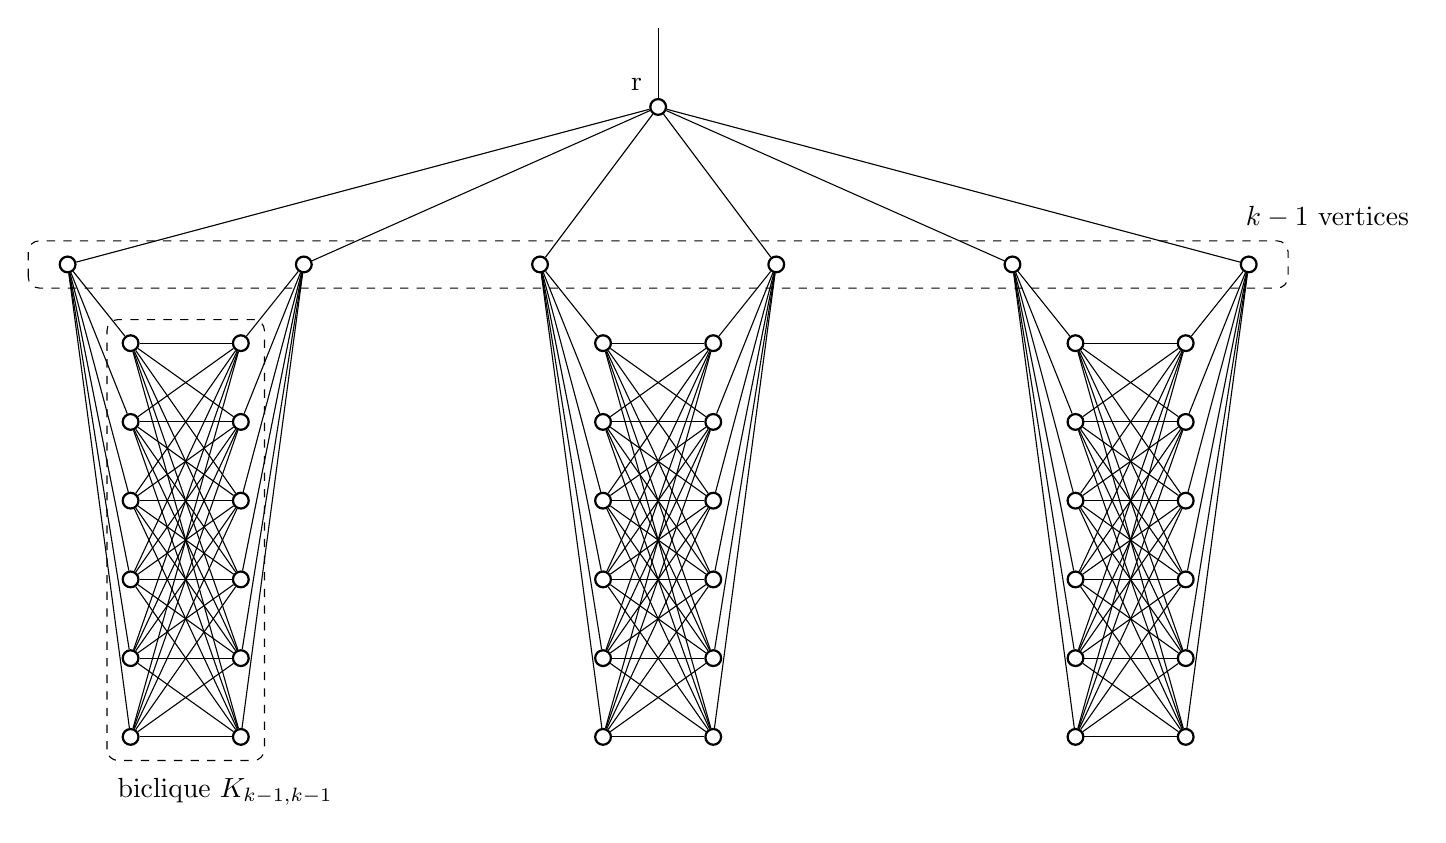
\begin{tikzpicture}
    % Nodes
    \node[small,label=above left:r] (r) at (7.5, 12) {};
    \foreach \i in {1,...,6} {
      \node[small] (x\i) at (-3 + 3 * \i, 10) {};
      \foreach \j in {1,...,3} {
        \node[small] (y\j\i) at (-5.2 + 6 * \j, 3 + \i) {};
        \node[small] (z\j\i) at (-3.8 + 6 * \j, 3 + \i) {};
      }
    }
    % Edges
    \draw (r) -- (7.5,13);
    \foreach \i in {1,...,6} {
      \draw (r) -- (x\i);
      \draw (x1) -- (y1\i);
      \draw (x2) -- (z1\i);
      \draw (x3) -- (y2\i);
      \draw (x4) -- (z2\i);
      \draw (x5) -- (y3\i);
      \draw (x6) -- (z3\i);
      \foreach \j in {1,...,6} {
        \foreach \k in {1,...,3} \draw (y\k\i) -- (z\k\j);
      }
    }
    % Annotations
    \draw[rounded corners, dashed] (-0.5, 9.7) rectangle ++ (16, 0.6);
    \node at (16, 10.6) {$k-1$ vertices};
    \draw[rounded corners, dashed] (0.5, 3.7) rectangle ++ (2, 5.6);
    \node at (2,3.3) {biclique $K_{k-1,k-1}$};
  \end{tikzpicture}
  \caption{$K_3$-free $k$-regular gadget.}
  \label{fig:regular-gadget}
\end{figure}
